% ============================================================
%  DUMMY PRESENTATION TEMPLATE  --  ASTRA 2026 theme
%  Topic: Machine-learning design of Rayleigh-wave metamaterial cloaks
%  Built on: beamerthemeASTRA.sty  (same folder)
%  Companion paper: ../wavemotion-paper/elsarticle-template-num.tex
%  Latent-space note:  ../latent_optim/latent_optim_short.tex
%
%  NOTE: logos (iist_logo.png, Astra_logo.png, ASTRA_Banner.png) are
%        intentionally NOT included yet -- add them to this folder later.
%        Everything else is placeholder/dummy content: swap author names,
%        trim slides to the 10-minute limit, and replace captions as needed.
%
%  Compile: pdflatex presentation  (x2, for nav)   or   latexmk -pdf presentation
% ============================================================

\documentclass[aspectratio=169, 10pt]{beamer}
\usepackage{newtxtext}
\usepackage{newtxmath}
\usepackage{beamerthemeASTRA}   % custom theme (in same folder)

% ---- Additional packages ----
\usepackage{amsmath, amssymb, bm}
\usepackage{booktabs}
\usepackage{multicol}
\usepackage{caption}
\usepackage{hyperref}
\usepackage[loadonly]{enumitem}
\usepackage{array}
\usepackage{pifont}
\usepackage{ragged2e}
\usepackage{tikz}
\usetikzlibrary{positioning,arrows.meta,fit,backgrounds,shapes.geometric}

% ---- Find figures from the paper and the latent-optim note ----
\graphicspath{{./}{../wavemotion-paper/figures/}{../latent_optim/}{./logos/}}

% ---- Hyperlink colours ----
\hypersetup{colorlinks=true, urlcolor=ASTRAaccent, linkcolor=ASTRAblue, citecolor=ASTRAblue}

% ---- Math shorthands (mirror the paper) ----
\newcommand{\mbf}[1]{\mathbf{#1}}
\newcommand{\mcl}[1]{\mathcal{#1}}
\newcommand{\Ceff}{\mbf{c}^{\mathrm{eff}}}
\newcommand{\Cfcm}{\mbf{C}_{\mathrm{4CM}}}
\newcommand{\uref}{\mbf{u}_{\mathrm{ref}}}

% ---- Reusable "takeaway" banner (orange alert box) ----
\newcommand{\takeaway}[1]{%
  \vspace{0.3em}%
  \begin{beamercolorbox}[wd=\textwidth, rounded=true, sep=6pt]{block body alerted}
    \small\textbf{\textcolor{ASTRAorange}{\ding{228}\ Takeaway.}}~#1
  \end{beamercolorbox}}

% ---- Reusable "big number" macro ----
\newcommand{\bignum}[2]{{\color{ASTRAorange}\bfseries #1}\,{\footnotesize #2}}

% ============================================================
%  PAPER METADATA
% ============================================================
\title{Machine-Learning Design of\\ Broadband Rayleigh-Wave Carpet Cloaks\\
       {\large under Microstructure Realisability Constraints}}

\author{%
  \textbf{\textcolor{ASTRAaccent}{David Aznaurov}}%
  \texorpdfstring{\textcolor{ASTRAgold}{\textsuperscript{*a}}}{*a}\textcolor{ASTRAnavy}{,~}%
  \textbf{\textcolor{ASTRAnavy}{Davit Piliposyan}}%
  \texorpdfstring{\textcolor{ASTRAgold}{\textsuperscript{a}}}{a}\textcolor{ASTRAnavy}{,~}%
  \textbf{\textcolor{ASTRAnavy}{Sébastien Guenneau}}%
  \texorpdfstring{\textcolor{ASTRAgold}{\textsuperscript{b}}}{b}%
  % Small demarcation line (Gold)
  \\[0.4em]{\color{ASTRAgold}\rule{4cm}{0.6pt}}%
}

\setAffiliations{%
  \textsuperscript{a}Mathematical Modelling and Machine Learning, Institute of Mechanics NAS RA \\
  \textsuperscript{b}Department of Physics, Imperial College London%
}

\setCorrespondingAuthor{%
  *Presenting author: \href{mailto:}{david@mechins.sci.am}%
}

\setPaperID{}
\institute{METAMAT 2026, Ajaccio, France}
\date{20--24 July 2026}

% ============================================================
\begin{document}
% ============================================================

% ------------------------------------------------------------
%  SLIDE 1 -- Title
% ------------------------------------------------------------
\begin{frame}[plain]
  \titlepage
\end{frame}

% ------------------------------------------------------------
%  SLIDE 2 -- Outline
% ------------------------------------------------------------
\begin{frame}{Outline}
  \begin{columns}[T]
    \begin{column}{0.56\textwidth}
      \setbeamerfont{enumerate item}{size=\normalsize}
      \begin{enumerate}
        \setlength{\itemsep}{0.55em}
        \item {\normalsize The dream: a cloak for surface waves}
        \item {\normalsize The catch: exact cloaks are unbuildable}
        \item {\normalsize Idea: \emph{let a network find the material}}
        \item {\normalsize Four ML routes to a real structure}
          \begin{itemize}\footnotesize
            \item Neural-field material optimisation
            \item Unit-cell inverse design
            \item Guided-diffusion generation
            \item Latent-space search
          \end{itemize}
        \item {\normalsize Results, and how much survives fabrication}
      \end{enumerate}
    \end{column}
    \begin{column}{0.42\textwidth}
      \centering
      % FIGURE: teaser -- the realised single-material cloak
      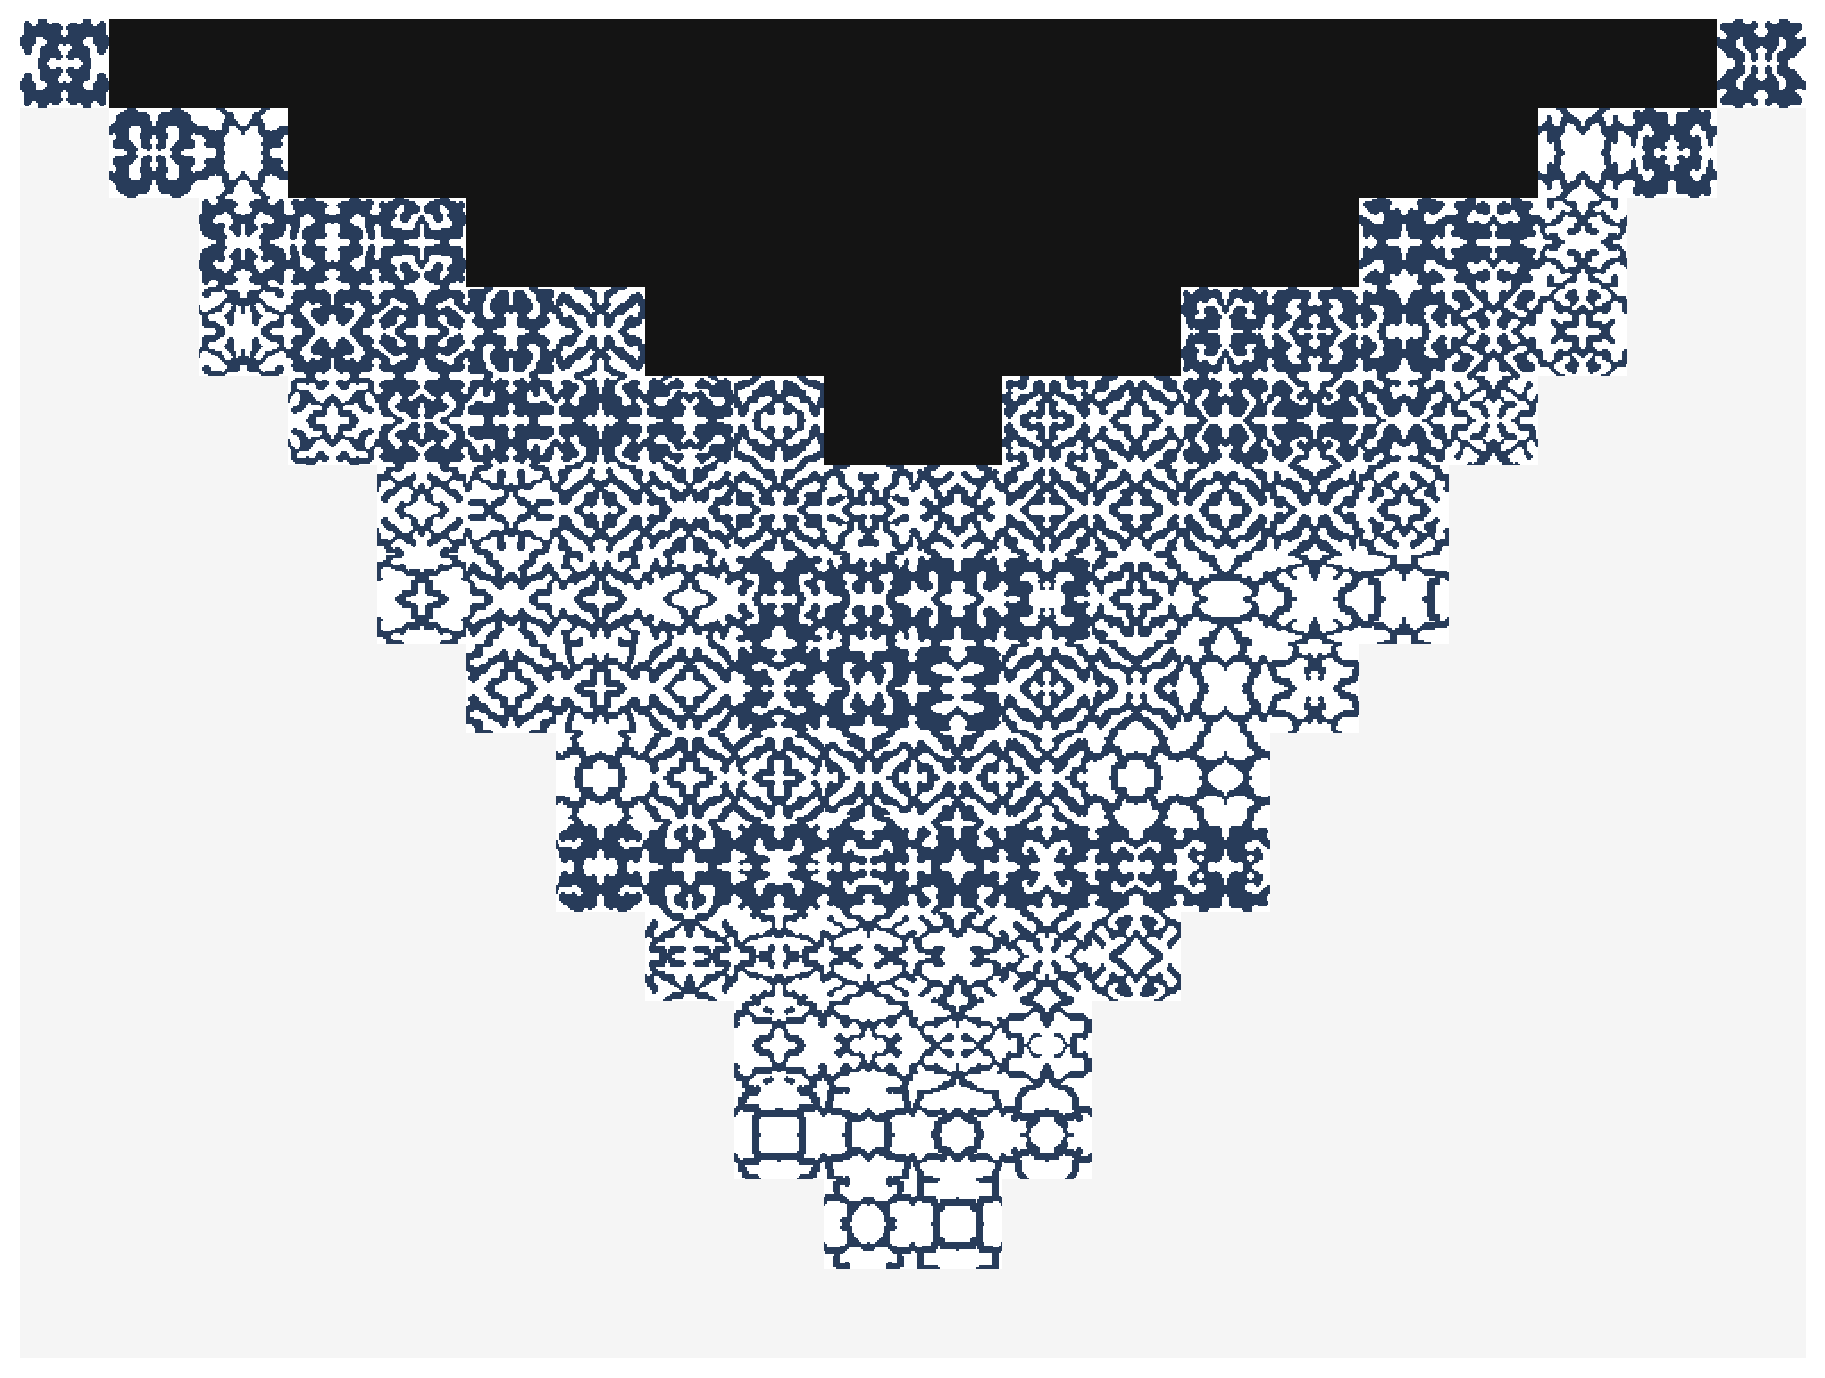
\includegraphics[width=\linewidth]{cloak_microstructure_diffusion.png}\\
      {\scriptsize A cloak made of \emph{one} material, patterned cell by cell.}
    \end{column}
  \end{columns}
\end{frame}

% ------------------------------------------------------------
%  SLIDE 3 -- Motivation
% ------------------------------------------------------------
\begin{frame}{Hiding from a surface wave}
  \begin{columns}[T]
    \begin{column}{0.50\textwidth}
      \begin{block}{The goal}
        \begin{itemize}
          \item A \textbf{Rayleigh wave} rolls along the free surface of a
                half-space. A surface \emph{notch} scatters it and casts a
                downstream shadow.
          \item A \textbf{carpet cloak} is a coating that makes the surface
                wave behave as if the notch were not there.
          \item Applications: seismic protection, surface-acoustic-wave
                devices, non-destructive testing.
        \end{itemize}
      \end{block}
      \takeaway{We want a coating, buildable from \emph{ordinary materials},
        that restores the surface wavefield beyond the defect.}
    \end{column}
    \begin{column}{0.48\textwidth}
      \centering
      % FIGURE: problem-setup.png  (domain + PML + point source + triangular cloak)
      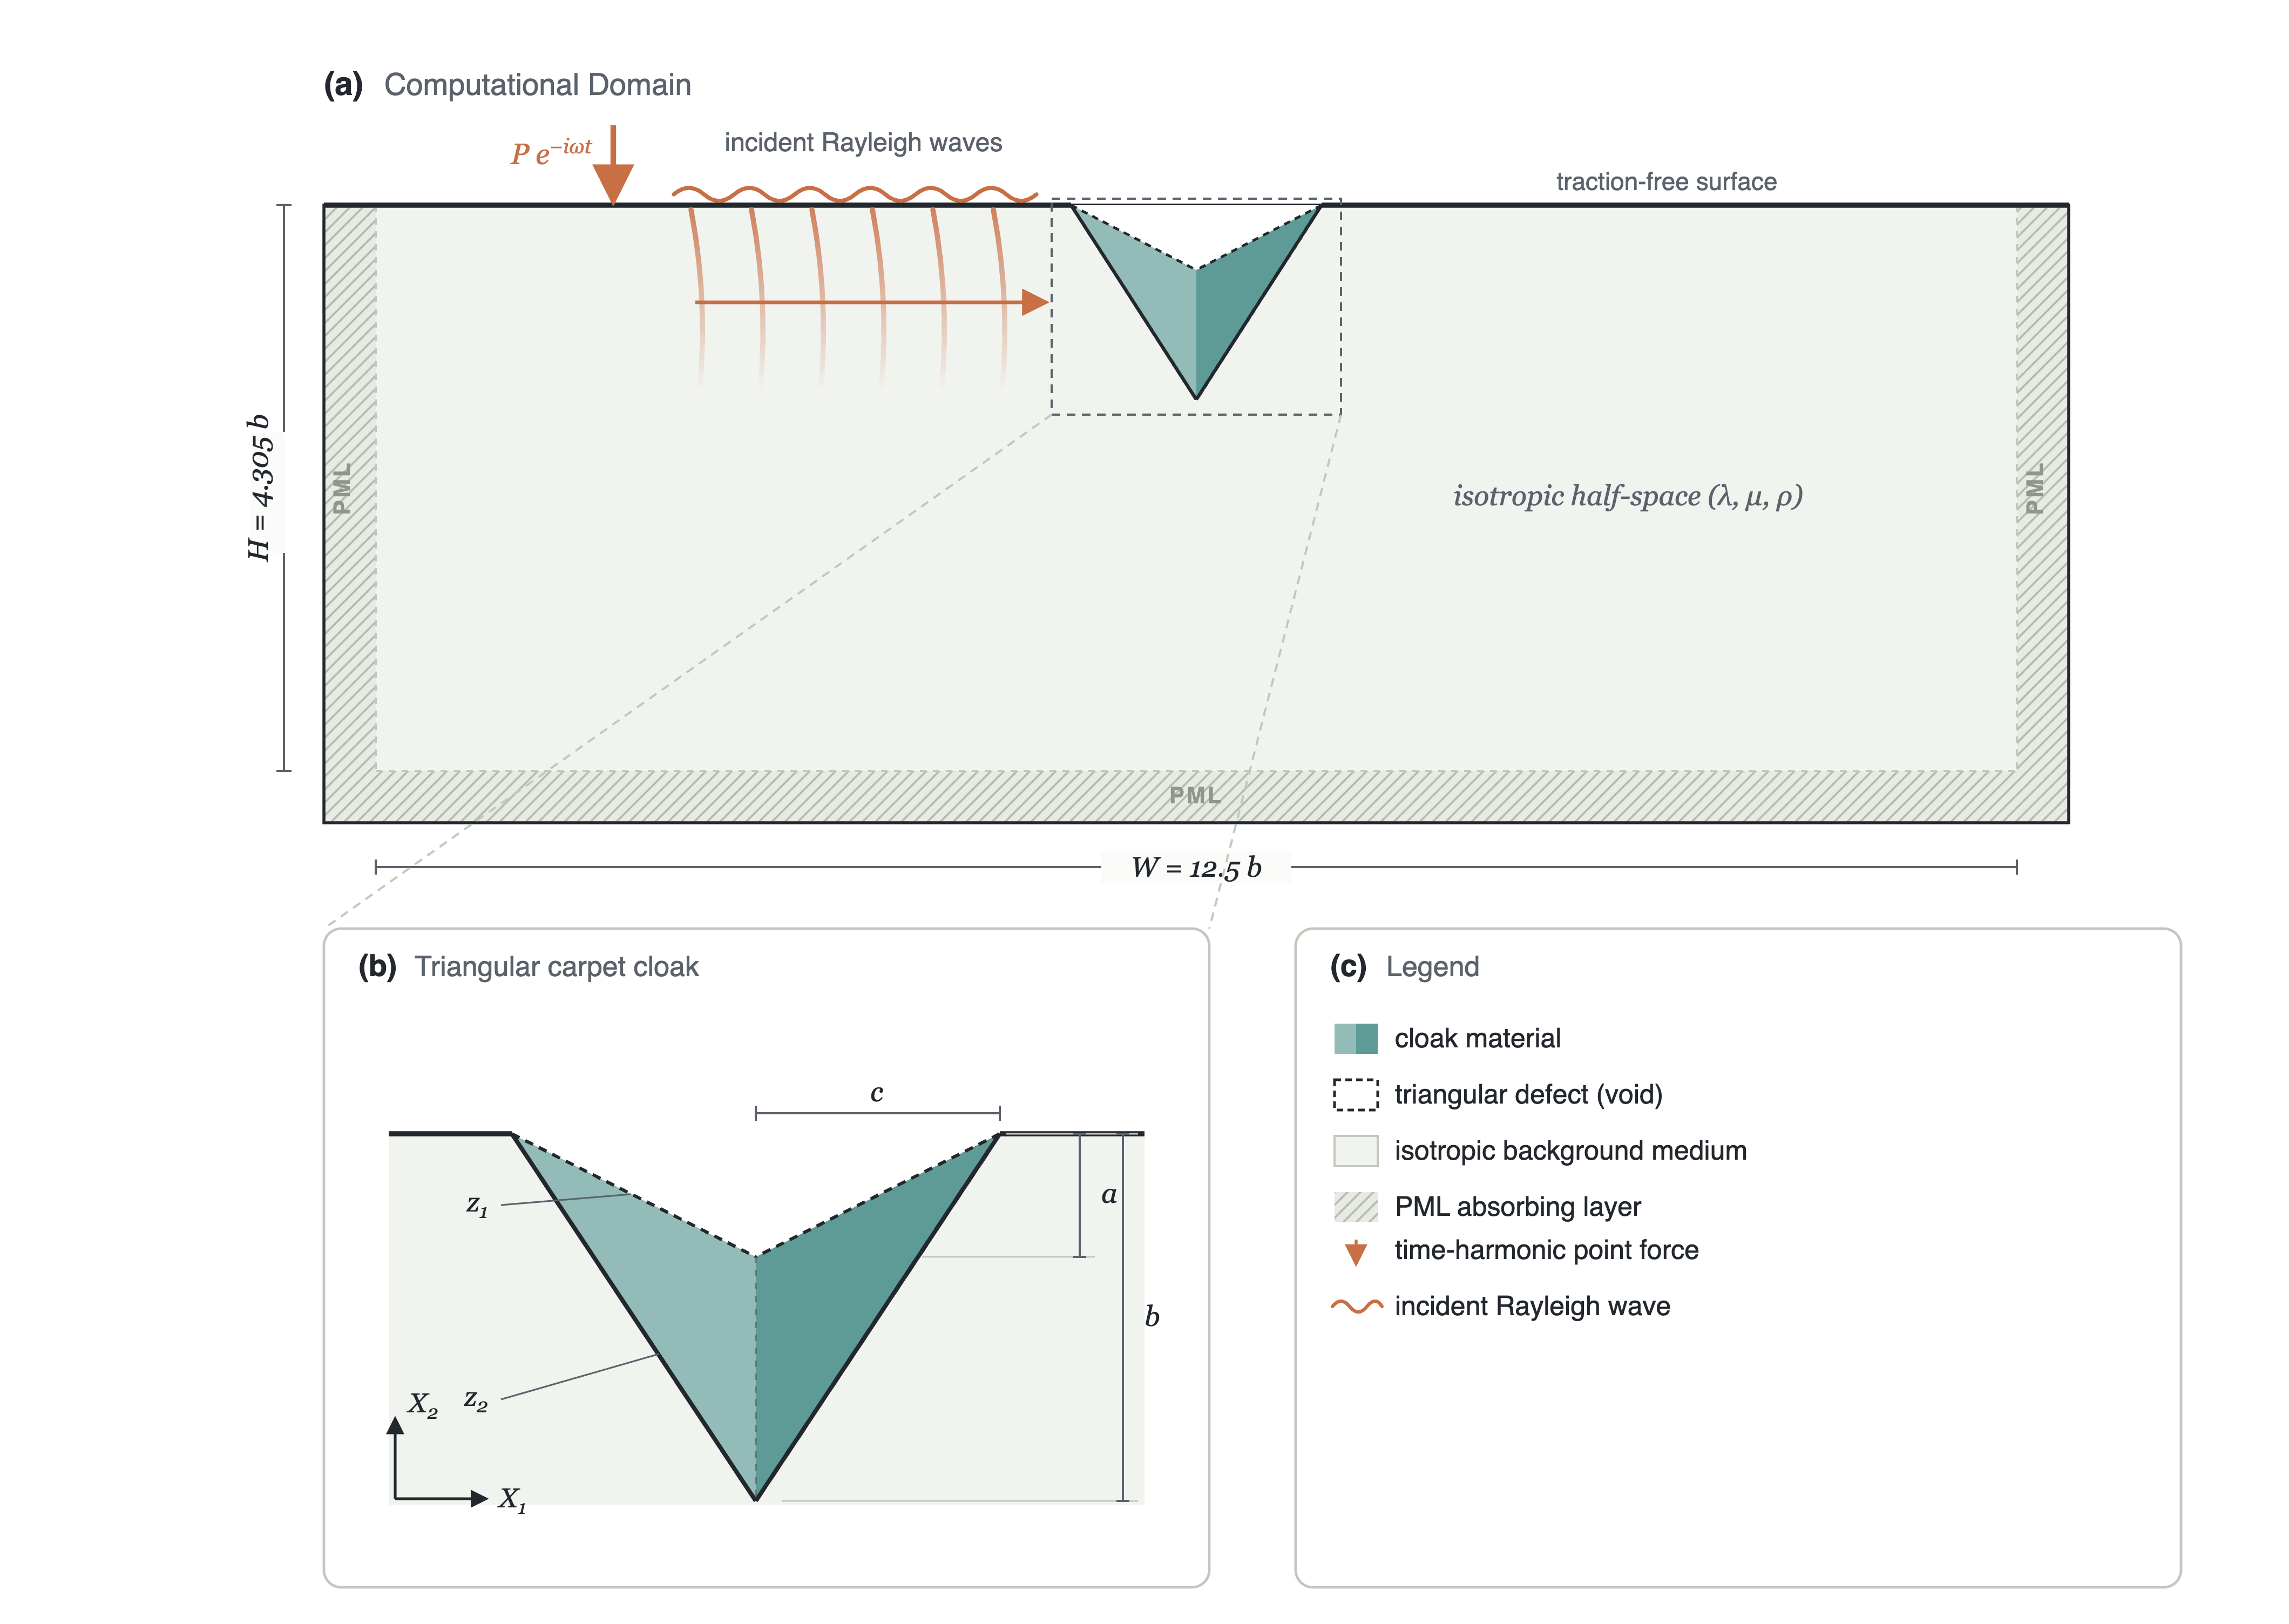
\includegraphics[width=\linewidth]{problem-setup.png}\\
      {\scriptsize Half-space, PML boundaries, a time-harmonic point source,
      and the triangular cloak over the notch.}
    \end{column}
  \end{columns}
\end{frame}

% ------------------------------------------------------------
%  SLIDE 4 -- Objectives / Contributions
% ------------------------------------------------------------
\begin{frame}{What we built}
  \begin{block}{Objective}
    Cast carpet-cloak design as a \textbf{PDE-constrained optimisation} solved
    by a coordinate \textbf{neural field} through a \textbf{differentiable
    finite-element} wave solver, and carry the design all the way to a
    fabricable single-material microstructure.
  \end{block}
  \vspace{0.2em}
  \begin{columns}[T]
    \begin{column}{0.49\textwidth}
      \begin{enumerate}\footnotesize
        \item[\ding{202}] \textbf{Neural-field material optimisation} --
              the main pipeline (Sec.~3).
        \item[\ding{203}] \textbf{Unit-cell inverse design} with a neural field.
        \item[\ding{204}] \textbf{Guided-diffusion} generation of unit cells.
        \item[\ding{205}] \textbf{Latent-space search} over a learned design manifold.
      \end{enumerate}
    \end{column}
    \begin{column}{0.49\textwidth}
      \begin{beamercolorbox}[wd=\textwidth, rounded=true, sep=7pt]{block body alerted}
        \centering\small
        Unconstrained design $\to$ \bignum{$\eta=0.99$}{} (near-ideal)\\[0.3em]
        Best \emph{fabricable} design $\to$ \bignum{$\approx\!97\%$}{ of ideal}\\[0.3em]
        {\scriptsize First microstructured Rayleigh-wave cloak from a common material.}
      \end{beamercolorbox}
    \end{column}
  \end{columns}
\end{frame}

% ------------------------------------------------------------
%  SLIDE 5 -- Transformation elasticity: the exact recipe
% ------------------------------------------------------------
\begin{frame}{Transformation elasticity: the exact cloak}
  A coordinate map $\mbf{x}=\Xi(\mbf{X})$, $\mbf{F}=\nabla_{\!X}\mbf{x}$,
  $J=\det\mbf{F}$, rewrites Navier's equation
  $\nabla_{\!x}\!\cdot(\Ceff:\nabla_{\!x}\mbf{u})=\rho^{\mathrm{eff}}\mbf{u}_{tt}$
  with the \textbf{Brun--Guenneau--Movchan} push-forward:
  \begin{equation*}
    c^{\mathrm{eff}}_{ijkl}=J^{-1}\,C_{IjKl}\,F_{iI}\,F_{kK},
    \qquad \rho^{\mathrm{eff}}=\rho\,J^{-1}.
  \end{equation*}
  \begin{columns}[T]
    \begin{column}{0.55\textwidth}
      \begin{block}{The obstruction (rigid statement)}
        \small The transformed tensor keeps the \emph{major} symmetry but
        breaks the \emph{minor} ones,
        \[
          c^{\mathrm{eff}}_{ijkl}=c^{\mathrm{eff}}_{klij},
          \qquad
          c^{\mathrm{eff}}_{ijkl}\neq c^{\mathrm{eff}}_{jikl}.
        \]
        Hence the ideal cloak is a \textbf{polar (Cosserat)} medium with a
        non-symmetric stress -- it lies \emph{outside} the class of ordinary
        Cauchy materials.
      \end{block}
    \end{column}
    \begin{column}{0.43\textwidth}
      \takeaway{The exact cloak is a theorem, not a blueprint. Our job is the
        \emph{best realisable approximation} inside the Cauchy class.}
    \end{column}
  \end{columns}
\end{frame}

% ------------------------------------------------------------
%  SLIDE 6 -- The triangular carpet cloak
% ------------------------------------------------------------
\begin{frame}{Why triangular? Two phases instead of a singularity}
  \begin{columns}[T]
    \begin{column}{0.52\textwidth}
      \small
      Pinched-carpet shear map (Chatzopoulos 2023). Its gradient is
      \emph{piecewise constant}:
      \begin{equation*}
        \mbf{F}=\begin{bmatrix}1&0\\ F_{21}&F_{22}\end{bmatrix},\quad
        F_{21}=\operatorname{sign}(X_1)\tfrac{a}{c},\quad
        F_{22}=\tfrac{b-a}{b}=J,
      \end{equation*}
      so the effective material is \textbf{uniform in each half} of the cloak
      and $\rho^{\mathrm{eff}}=\tfrac{b}{b-a}\rho$ is constant.
      \begin{itemize}
        \item No inner-boundary singularity (unlike radial blow-up cloaks).
        \item Ideal cloak $=$ just \textbf{two} mirror-image phases\ldots
        \item \ldots but \emph{three} minor-symmetry pairs are broken -- exactly
              what symmetrisation averages away by hand.
      \end{itemize}
    \end{column}
    \begin{column}{0.46\textwidth}
      \centering
      % FIGURE: triangular-cell-decomposition.png
      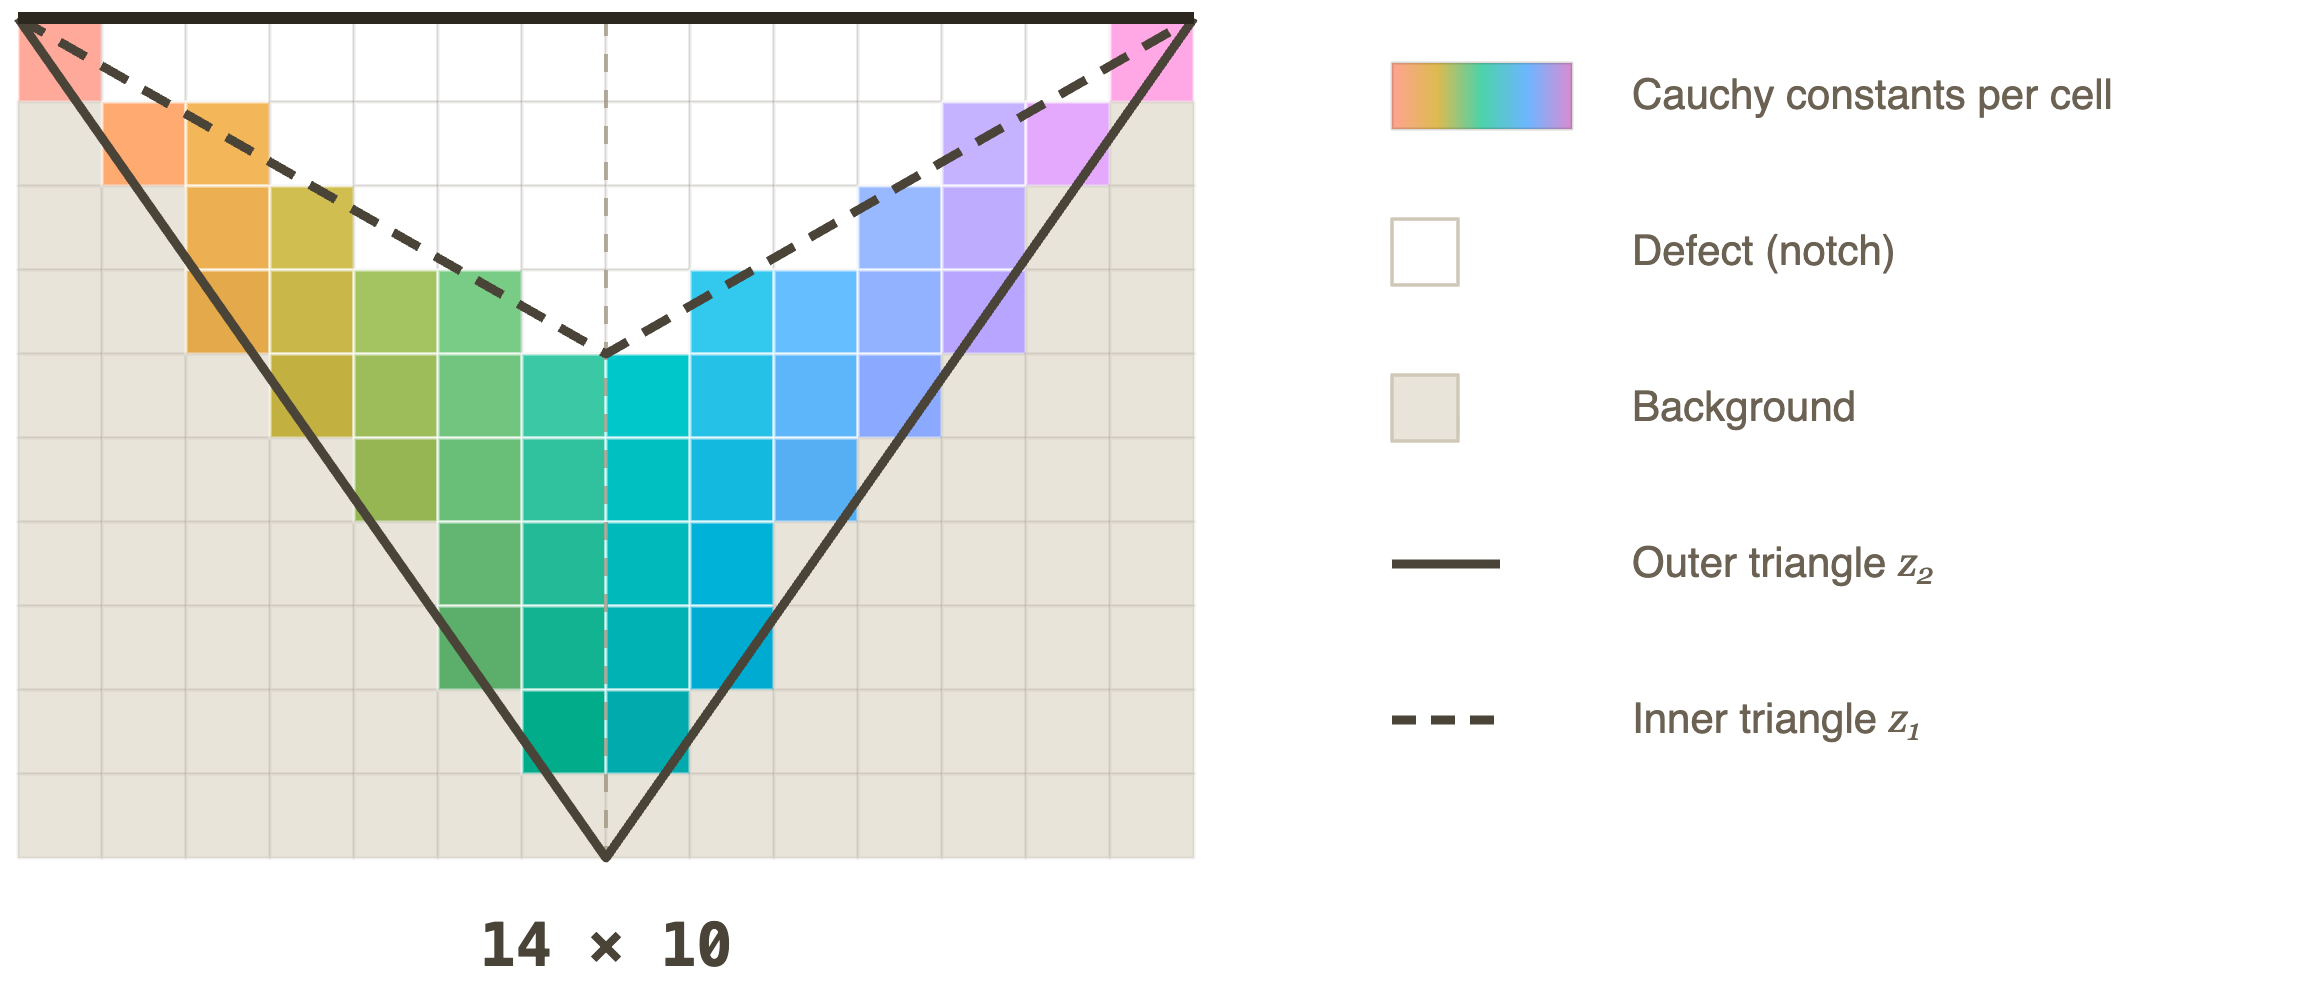
\includegraphics[width=0.92\linewidth]{triangular-cell-decomposition.png}\\
      {\scriptsize Cartesian $14\times10$ cell decomposition; only 46 cells fall
      inside the cloak (the active design variables).}
    \end{column}
  \end{columns}
\end{frame}

% ------------------------------------------------------------
%  SLIDE 7 -- Reformulation as optimisation
% ------------------------------------------------------------
\begin{frame}{From a broken theorem to an optimisation problem}
  \begin{columns}[T]
    \begin{column}{0.53\textwidth}
      \begin{block}{Design class: orthotropic Cauchy (4CM)}
        \small
        Square $D_2$-symmetric cells force $C_{16}=C_{26}=0$:
        \[
          \Cfcm=\begin{bmatrix}C_{11}&C_{12}&0\\ C_{12}&C_{22}&0\\ 0&0&C_{66}\end{bmatrix}\succ 0,
          \quad (+\,\rho).
        \]
        Four moduli $+$ density \emph{per cell} are the design variables.
      \end{block}
    \end{column}
    \begin{column}{0.45\textwidth}
      \begin{block}{Objective: phase-invariant magnitude error}
        \small
        \[
          \mcl{L}_{\mathrm{cloak}}(\theta)=\frac{1}{|\mcl{B}|}\int_{\mcl{B}}
          \!\Big(\tfrac{|\mbf{u}_{\mathrm{cloak}}|}{|\uref|}-1\Big)^{2}dA
        \]
        over a near-surface strip $\mcl{B}$ downstream of the cloak.
      \end{block}
    \end{column}
  \end{columns}
  \vspace{0.2em}
  \begin{center}\small
    Report card: the \textbf{cloak ratio}\quad
    $\displaystyle \eta=\frac{\langle|\mbf{u}|\rangle}{\langle|\uref|\rangle}\to 1$
    \quad(perfect cloak).
  \end{center}
  \takeaway{Magnitudes, not complex fields: a wave routed around the notch is
    allowed to arrive with a benign phase lag.}
\end{frame}

% ------------------------------------------------------------
%  SLIDE 8 -- Methodology overview (3 columns)
% ------------------------------------------------------------
\begin{frame}{Methodology: one differentiable pipeline}
  \begin{methodcols}
    \methodcol{\ding{202}~Represent}{%
      \begin{itemize}
        \item A coordinate MLP $\Phi_\theta$ \emph{is} the material field.
        \item Outputs $(\Cfcm,\rho)$ per cell.
        \item Smoothness set by Fourier features.
      \end{itemize}%
    }
    \methodcol{\ding{203}~Solve \& differentiate}{%
      \begin{itemize}
        \item Frequency-domain JAX-FEM wave solve.
        \item Gradients via the implicit \textbf{adjoint} of the linear solve.
        \item End-to-end $\partial\mcl{L}/\partial\theta$.
      \end{itemize}%
    }
    \methodcol{\ding{204}~Realise}{%
      \begin{itemize}
        \item Project onto a \textbf{realisability manifold}.
        \item Fill each cell with a solid/void microstructure.
        \item Inverse design $/$ diffusion $/$ latent search.
      \end{itemize}%
    }
  \end{methodcols}
  \vspace{0.3em}
  \begin{center}
    % Simple TikZ dataflow (self-contained; no external image needed)
    \begin{tikzpicture}[font=\scriptsize,>={Latex[length=2mm]},node distance=5mm,
        box/.style={draw=ASTRAblue,fill=ASTRAbglight,rounded corners=2pt,thick,
                    inner sep=4pt,align=center,minimum height=8mm}]
      \node[box] (xy)  {cell coords\\$(x,y)$};
      \node[box,right=of xy] (nf) {neural field\\$\Phi_\theta$};
      \node[box,right=of nf] (mat) {material\\$(\Cfcm,\rho)$};
      \node[box,right=of mat] (fem) {JAX-FEM\\wave solve};
      \node[box,right=of fem] (loss) {cloak loss\\$\mcl{L}$};
      \draw[->,thick,ASTRAnavy] (xy)--(nf);
      \draw[->,thick,ASTRAnavy] (nf)--(mat);
      \draw[->,thick,ASTRAnavy] (mat)--(fem);
      \draw[->,thick,ASTRAnavy] (fem)--(loss);
      \draw[->,thick,dashed,ASTRAorange] (loss.south) to[out=-90,in=-90]
            node[below,midway]{adjoint gradient $\partial\mcl{L}/\partial\theta$} (nf.south);
    \end{tikzpicture}
  \end{center}
\end{frame}

% ------------------------------------------------------------
%  SLIDE 9 -- Method 1: neural-field material optimisation
% ------------------------------------------------------------
\begin{frame}{\ding{202} Method 1 -- Neural-field material optimisation}
  \begin{columns}[T]
    \begin{column}{0.50\textwidth}
      \small
      Reparameterise the material field by a coordinate MLP
      \[
        \Phi_\theta:(x,y)\mapsto(\Cfcm(x,y),\,\rho(x,y)),
      \]
      applied as a \textbf{multiplicative residual} around a physical prior:
      \[
        \Cfcm=\Cfcm^{(0)}\odot\big(1+\epsilon\,\Phi^{(C)}_\theta\big).
      \]
      \begin{itemize}
        \item $\tanh$ MLP, 4 layers, Fourier positional encoding.
        \item Relative perturbation is scale-uniform across moduli.
        \item Smoothness is \emph{built in} -- no neighbour penalty needed.
      \end{itemize}
    \end{column}
    \begin{column}{0.49\textwidth}
      \centering
      % FIGURE: ml-pipeline.png  (the neural-field design pipeline schematic)
      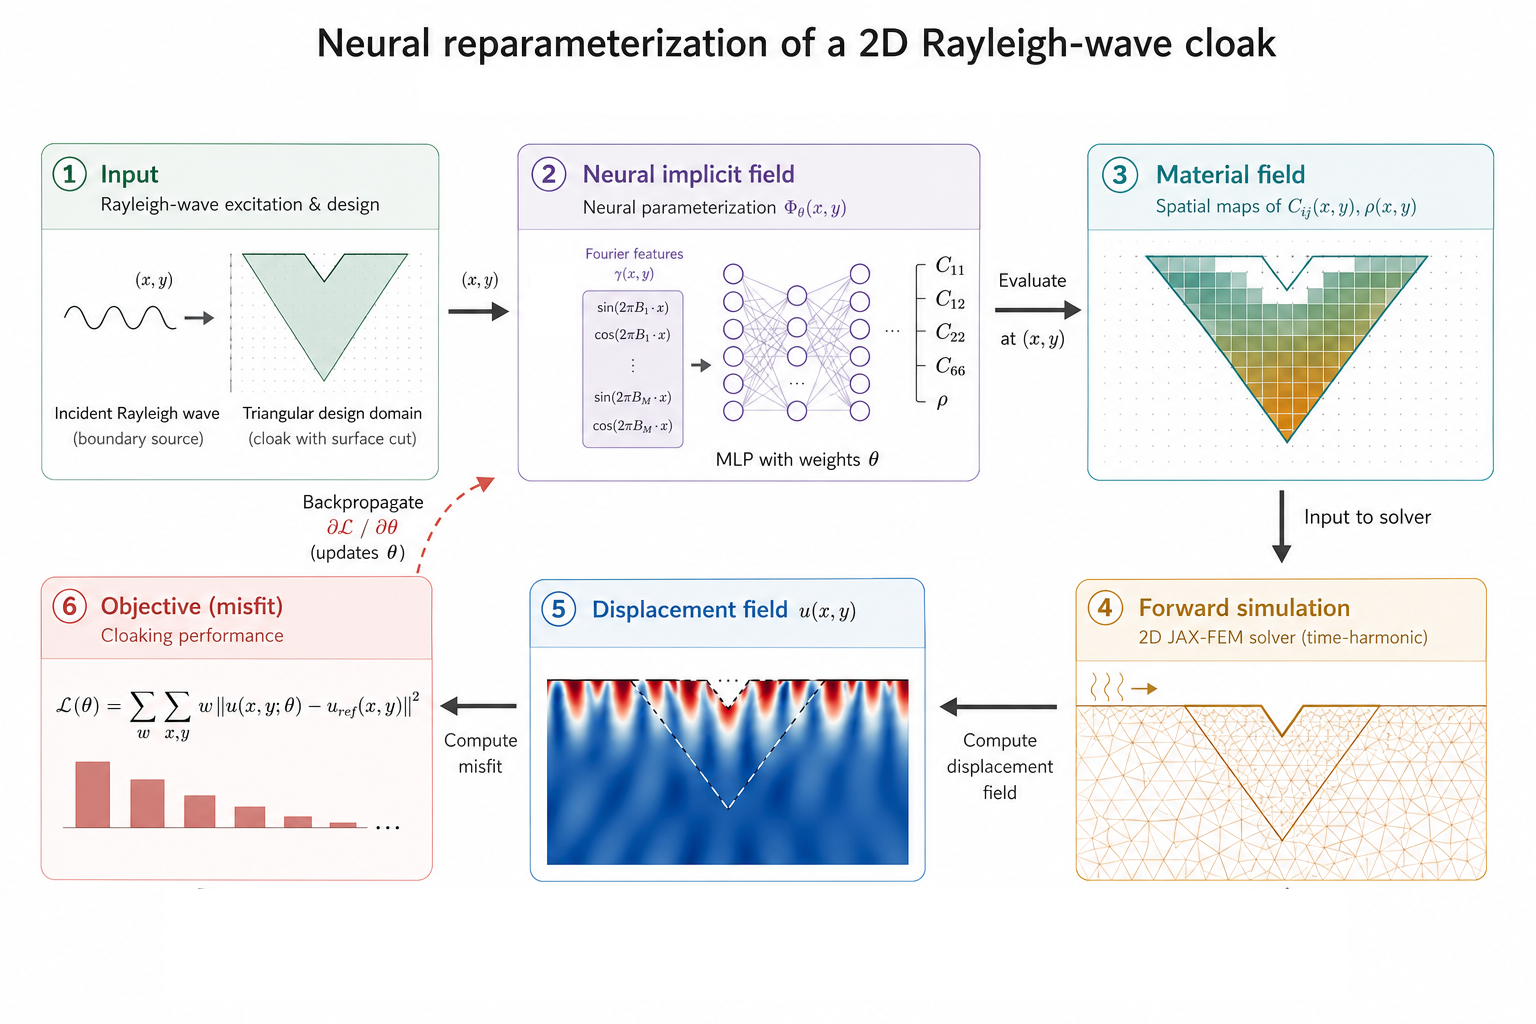
\includegraphics[width=\linewidth]{ml-pipeline.png}\\
      {\scriptsize Coordinates $\to$ Fourier encoding $\to$ MLP $\to$
      $(\Cfcm,\rho)$ $\to$ FEM $\to$ loss, differentiated back to $\theta$.}
    \end{column}
  \end{columns}
  \takeaway{The network is the material. Design $=$ training its weights against
    a wave-physics loss.}
\end{frame}

% ------------------------------------------------------------
%  SLIDE 10 -- Method 1b: admissible-by-construction decoding
% ------------------------------------------------------------
\begin{frame}{\ding{202} Admissible \emph{by construction}: the decoding map}
  \small
  Raw outputs $\mbf{r}=(r_{11},r_{22},r_{66},r_{12})$ are decoded so every design
  is a valid Cauchy tensor -- no penalty policing after the fact.
  \begin{columns}[T]
    \begin{column}{0.33\textwidth}
      \begin{block}{Positivity}
        \[ C_{ii}=C_{ii}^{(0)}e^{\epsilon r_{ii}} \]
        Log-space $\Rightarrow C_{ii}>0$ for any real $r_{ii}$.
      \end{block}
    \end{column}
    \begin{column}{0.33\textwidth}
      \begin{block}{Bounded anisotropy}
        \[ g_b=\tfrac12\log R\,\tanh\!\Big(\tfrac{g}{\frac12\log R}\Big) \]
        confines $C_{11}/C_{22}\in[1/R,R]$, $R=30$.
      \end{block}
    \end{column}
    \begin{column}{0.33\textwidth}
      \begin{block}{PD coupling}
        \[ C_{12}=\rho_c\sqrt{C_{11}C_{22}} \]
        $\rho_c=\kappa\tanh(r_{12}{+}\phi_0)$, $\kappa=0.99$
        $\Rightarrow\det\!>\!0$.
      \end{block}
    \end{column}
  \end{columns}
  \takeaway{A smooth, everywhere-differentiable surjection onto the set of
    positive-definite, bounded-anisotropy tensors: the optimiser can never leave
    the realisable class.}
\end{frame}

% ------------------------------------------------------------
%  SLIDE 11 -- Results I: single frequency
% ------------------------------------------------------------
\begin{frame}{Results I -- one material already beats symmetrisation}
  \begin{columns}[T]
    \begin{column}{0.44\textwidth}
      \centering\scriptsize
      \captionof*{table}{Cloak ratio $\eta$ at $f^\star=2.0$}
      \begin{tabular}{@{}lc@{}}
        \toprule
        Configuration & $\eta$ \\
        \midrule
        Obstacle (no cloak)            & $0.37$ \\
        Symmetrised ideal (Chatz.\ 2023) & $0.63$ \\
        \textbf{Single optimised 4CM}  & $\mathbf{0.86}$ \\
        $2\times2$ (four materials)    & $0.96$ \\
        \textbf{$14\times10$ grid (46 cells)} & $\mathbf{0.99}$ \\
        \midrule
        Ideal continuous polar $\Ceff$ & $0.999$ \\
        \bottomrule
      \end{tabular}
      \vspace{0.4em}
      \par{\scriptsize Depth beats width: subdividing in depth helps far more
      than along propagation.}
    \end{column}
    \begin{column}{0.55\textwidth}
      \centering
      % FIGURE: single_freq_14x10_re_mag.png  (ref / notch / ideal / optimised)
      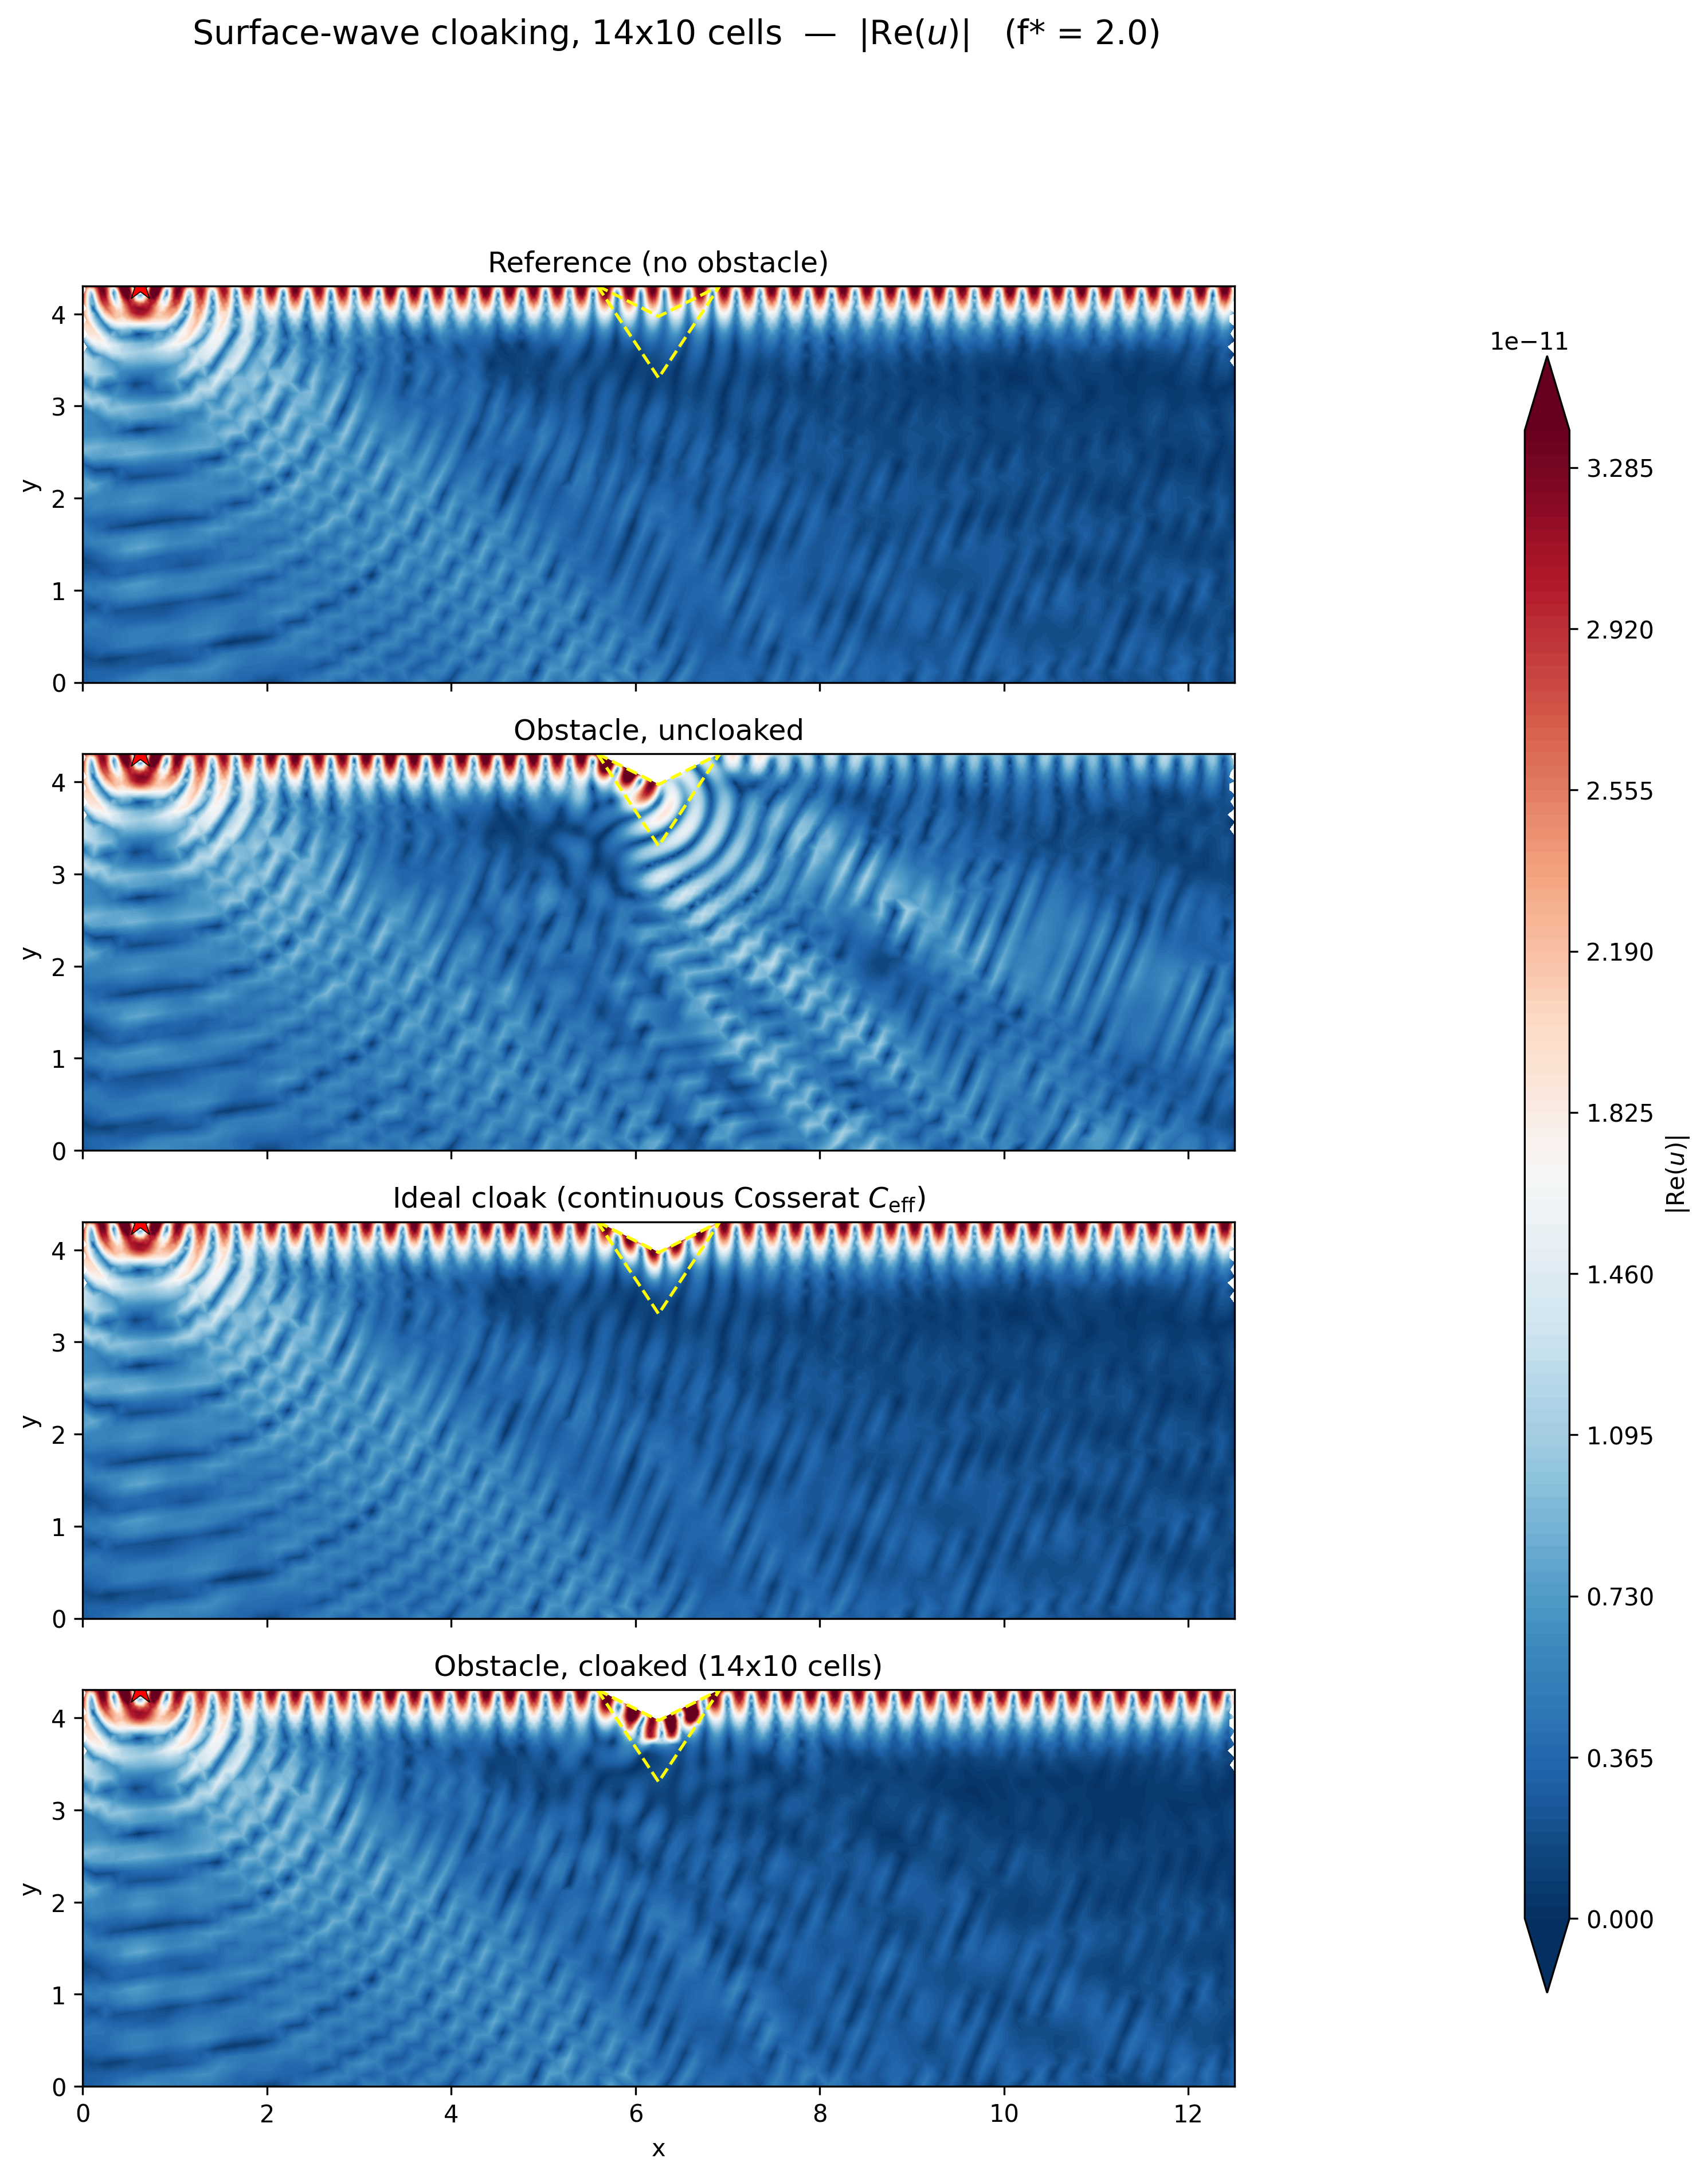
\includegraphics[width=\linewidth]{single_freq_14x10_re_mag.png}\\
      {\scriptsize Top$\to$bottom: reference, uncloaked notch (shadow!),
      ideal polar cloak, optimised $14\times10$ cloak ($\eta=0.99$).}
    \end{column}
  \end{columns}
  \takeaway{A single realisable material jumps $0.63\!\to\!0.86$; 46 cells reach
    $0.99$ -- essentially closing the gap to the ideal polar cloak.}
\end{frame}

% ------------------------------------------------------------
%  SLIDE 12 -- Results II: broadband
% ------------------------------------------------------------
\begin{frame}{Results II -- broadband: one design, a whole octave}
  \begin{columns}[T]
    \begin{column}{0.50\textwidth}
      \small
      Train a single neural field against a band of frequencies at once:
      \[
        \mcl{L}_{\mathrm{band}}(\theta)=
        \frac{1}{\sum_{f}w_f}\sum_{f\in\mcl{S}}w_f\,\mcl{L}_{\mathrm{cloak}}(\theta;f).
      \]
      \begin{itemize}
        \item Band $f^\star\in[1,3]$, 7 frequencies, equal weights.
        \item Optional min--max variant flattens the worst case.
        \item Cost scales linearly in $|\mcl{S}|$; frequencies solved in parallel.
        \item Floquet--Bloch check: propagating modes, \emph{no} resonant band-gap
              trickery.
      \end{itemize}
    \end{column}
    \begin{column}{0.49\textwidth}
      \centering
      % FIGURE: multifreq_sweep.png
      
\includegraphics[width=\linewidth]{multifreq_sweep.png}\\
      {\scriptsize $\eta(f)$: broadband design (blue) holds $\approx0.96$ across
      the shaded training band; degrades gracefully outside it.}
    \end{column}
  \end{columns}
  \takeaway{The single-frequency narrowness was a limit of the \emph{objective},
    not the material class.}
\end{frame}

% ------------------------------------------------------------
%  SLIDE 13 -- Bridge: from tensors to structures
% ------------------------------------------------------------
\begin{frame}{From numbers to structures: the realisability problem}
  \begin{block}{The gap}
    \small Optimised cells carry a homogenised $(\Cfcm,\rho)$ that need not
    correspond to any manufacturable object. We must \emph{realise} each cell as
    a real two-phase (solid/void) microstructure.
  \end{block}
  \begin{columns}[T]
    \begin{column}{0.60\textwidth}
      \begin{enumerate}\footnotesize
        \item[\ding{202}] \textbf{Dataset:} $N\!\sim\!10^{6}$ binary
              $50\times50$ cells (cellular-automaton growth).
        \item[\ding{203}] \textbf{Homogenise:} periodic FEM $\to(\Cfcm,\rho_{\mathrm{eff}})$;
              $D_2$ symmetry $\Rightarrow$ exactly the 4CM form.
        \item[\ding{204}] \textbf{Prior:} fit a GMM; keep a log-density super-level
              set as the realisable manifold $\mcl{M}$.
        \item[\ding{205}] \textbf{Constrain:} add the manifold penalty during
              optimisation.
      \end{enumerate}
    \end{column}
    \begin{column}{0.39\textwidth}
      \begin{block}{Manifold penalty}
        \small
        \[
          \mcl{L}_{\mathrm{GMM}}=\sum_c\max\!\big(0,\ \tau-\log p_{\mathrm{GMM}}(\Cfcm^{c},\rho_c)\big)
        \]
        pulls every cell into $\mcl{M}$ without pinning it to one catalogue entry.
      \end{block}
    \end{column}
  \end{columns}
\end{frame}

% ------------------------------------------------------------
%  SLIDE 14 -- Method 2: unit-cell inverse design
% ------------------------------------------------------------
\begin{frame}{\ding{203} Method 2 -- Unit-cell inverse design (neural field)}
  \begin{columns}[T]
    \begin{column}{0.54\textwidth}
      \small
      Given a per-cell target $\mbf{y}=(\Cfcm,\rho)$, parameterise a
      \emph{continuous density field} over the $50\times50$ cell,
      $\hat\rho(x,y)=g_\phi(x,y)\in[0,1]$, and minimise
      \[
        \min_{\phi}\ \big\|\mcl{H}(\hat\rho_\phi)-\mbf{y}\big\|^2 + \lambda\,\mcl{R}_{\mathrm{conn}},
      \]
      where $\mcl{H}$ is the differentiable periodic-FEM homogenisation operator.
      \begin{itemize}
        \item Soft-to-hard schedule drives $\hat\rho\to\{0,1\}$.
        \item Connectivity penalty $\mcl{R}_{\mathrm{conn}}$ kills floating
              islands/voids.
        \item \textbf{Deterministic}: one locally optimal cell per target.
      \end{itemize}
    \end{column}
    \begin{column}{0.45\textwidth}
      \centering
      % FIGURE: cloak_microstructure_inverse.png  (tiled inverse-design cloak)
      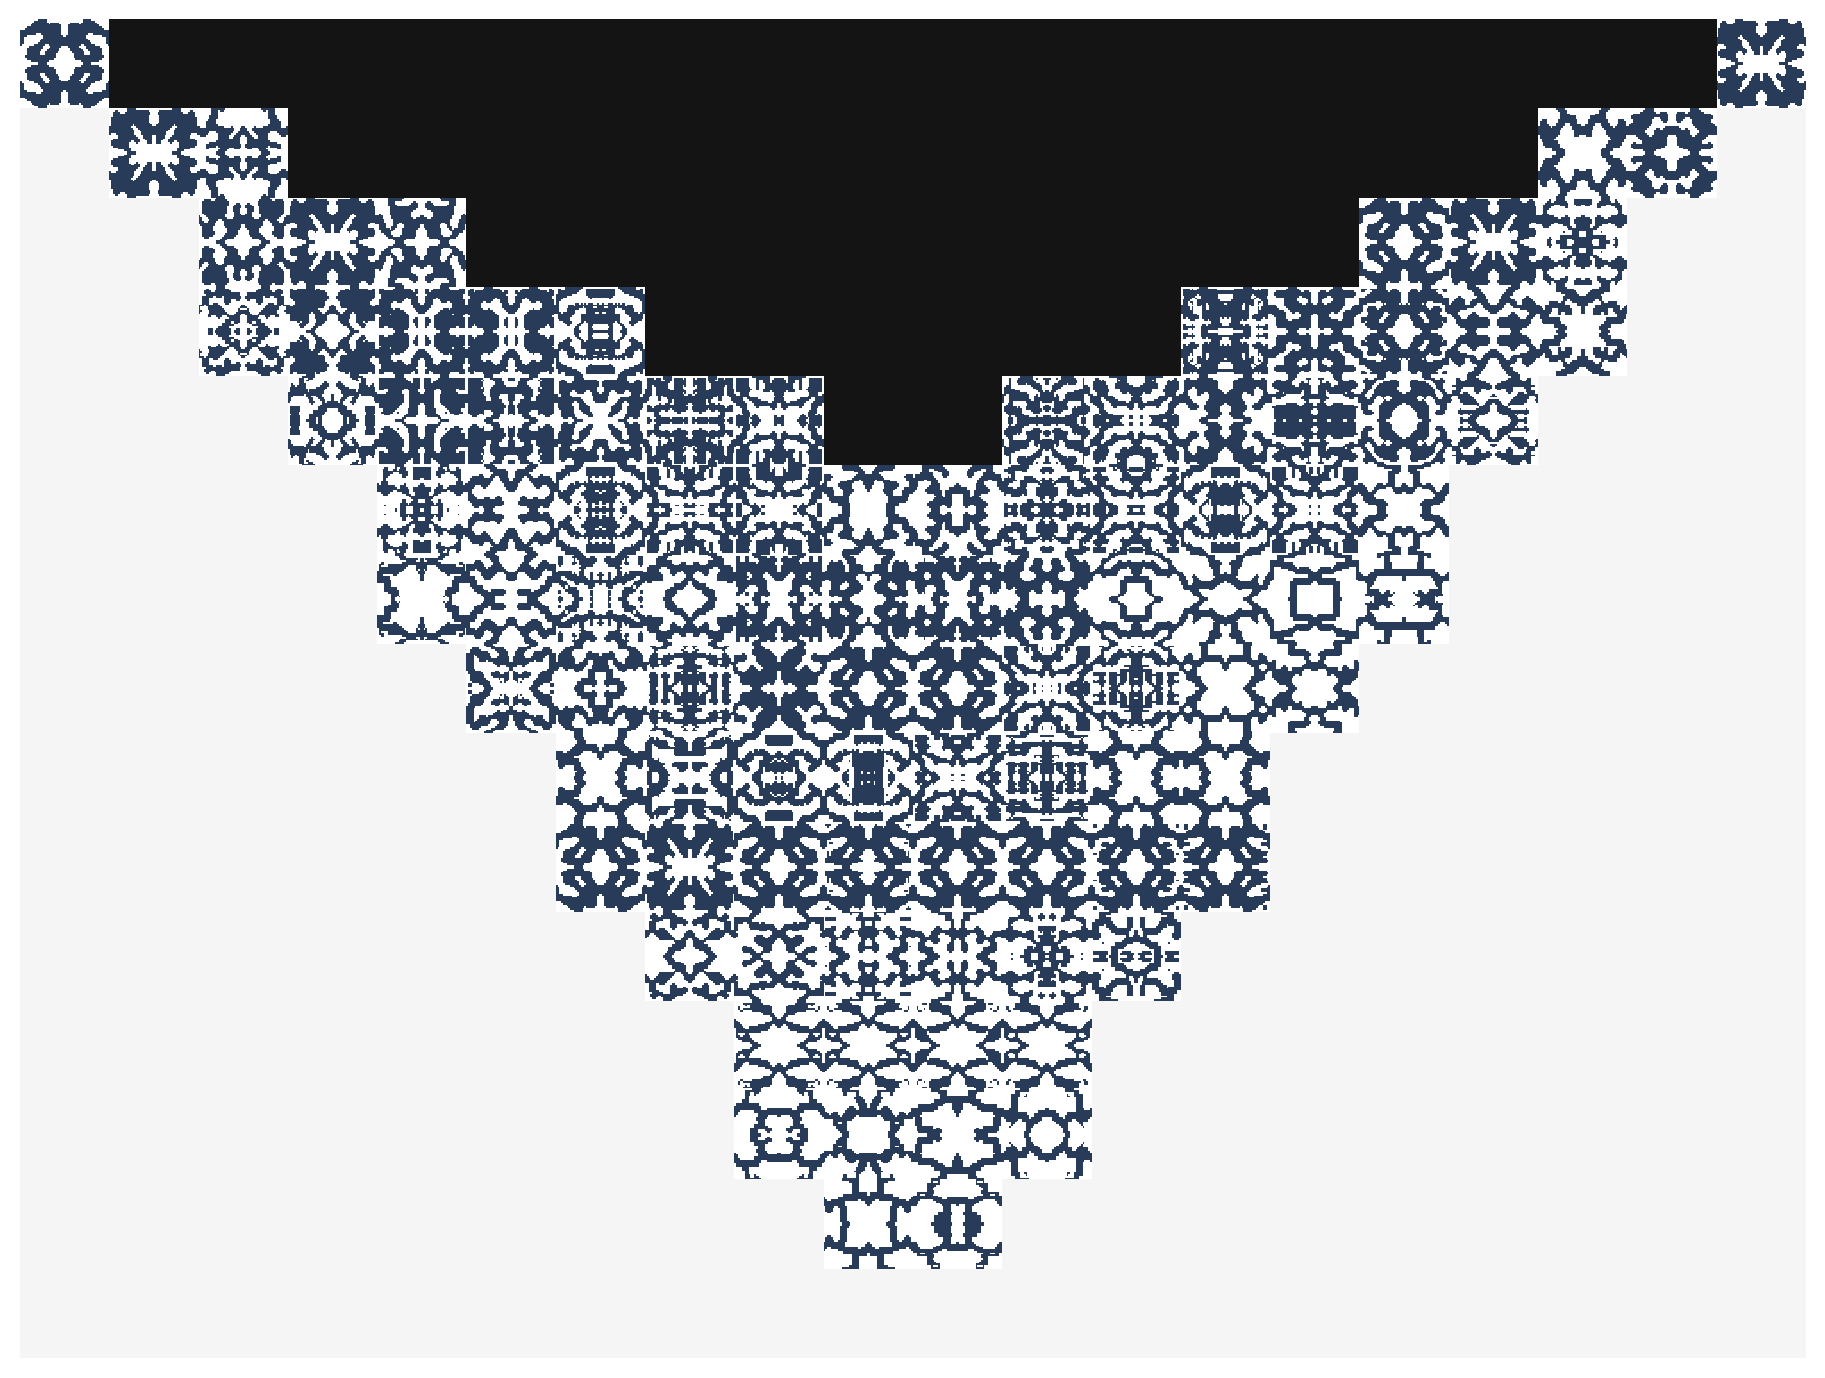
\includegraphics[width=\linewidth]{cloak_microstructure_inverse.png}\\
      {\scriptsize Inverse-design realisation: one cement phase, cell-varying
      void pattern tiled across the carpet.}
    \end{column}
  \end{columns}
\end{frame}

% ------------------------------------------------------------
%  SLIDE 15 -- Method 3: guided diffusion
% ------------------------------------------------------------
\begin{frame}{\ding{204} Method 3 -- Guided-diffusion generation}
  \begin{columns}[T]
    \begin{column}{0.54\textwidth}
      \small
      Train a \textbf{conditional denoising diffusion} model on the catalogue,
      \[
        \min_\theta\ \mathbb{E}_{t,\mbf{x}_0,\bm{\epsilon}}
        \big\|\bm{\epsilon}-\bm{\epsilon}_\theta(\mbf{x}_t,t,\mbf{y})\big\|^2,
        \quad \mbf{y}=(\Cfcm,\rho),
      \]
      then sample the reverse process $p_\theta(\mbf{x}_{t-1}\!\mid\!\mbf{x}_t,\mbf{y})$.
      Because sampling is stochastic, draw $N$ candidates and keep the closest:
      \[
        \mbf{x}^\star=\arg\min_{n=1..N}\ \big\|\mcl{H}(\mbf{x}^{(n)})-\mbf{y}\big\|
        \quad(\textbf{best-of-}N).
      \]
      \begin{itemize}
        \item Prior keeps every sample \emph{on} the manufacturable manifold.
        \item Explores a diverse set of realisations per target.
      \end{itemize}
    \end{column}
    \begin{column}{0.45\textwidth}
      \centering
      % FIGURE: cloak_microstructure_diffusion.png  (tiled diffusion cloak)
      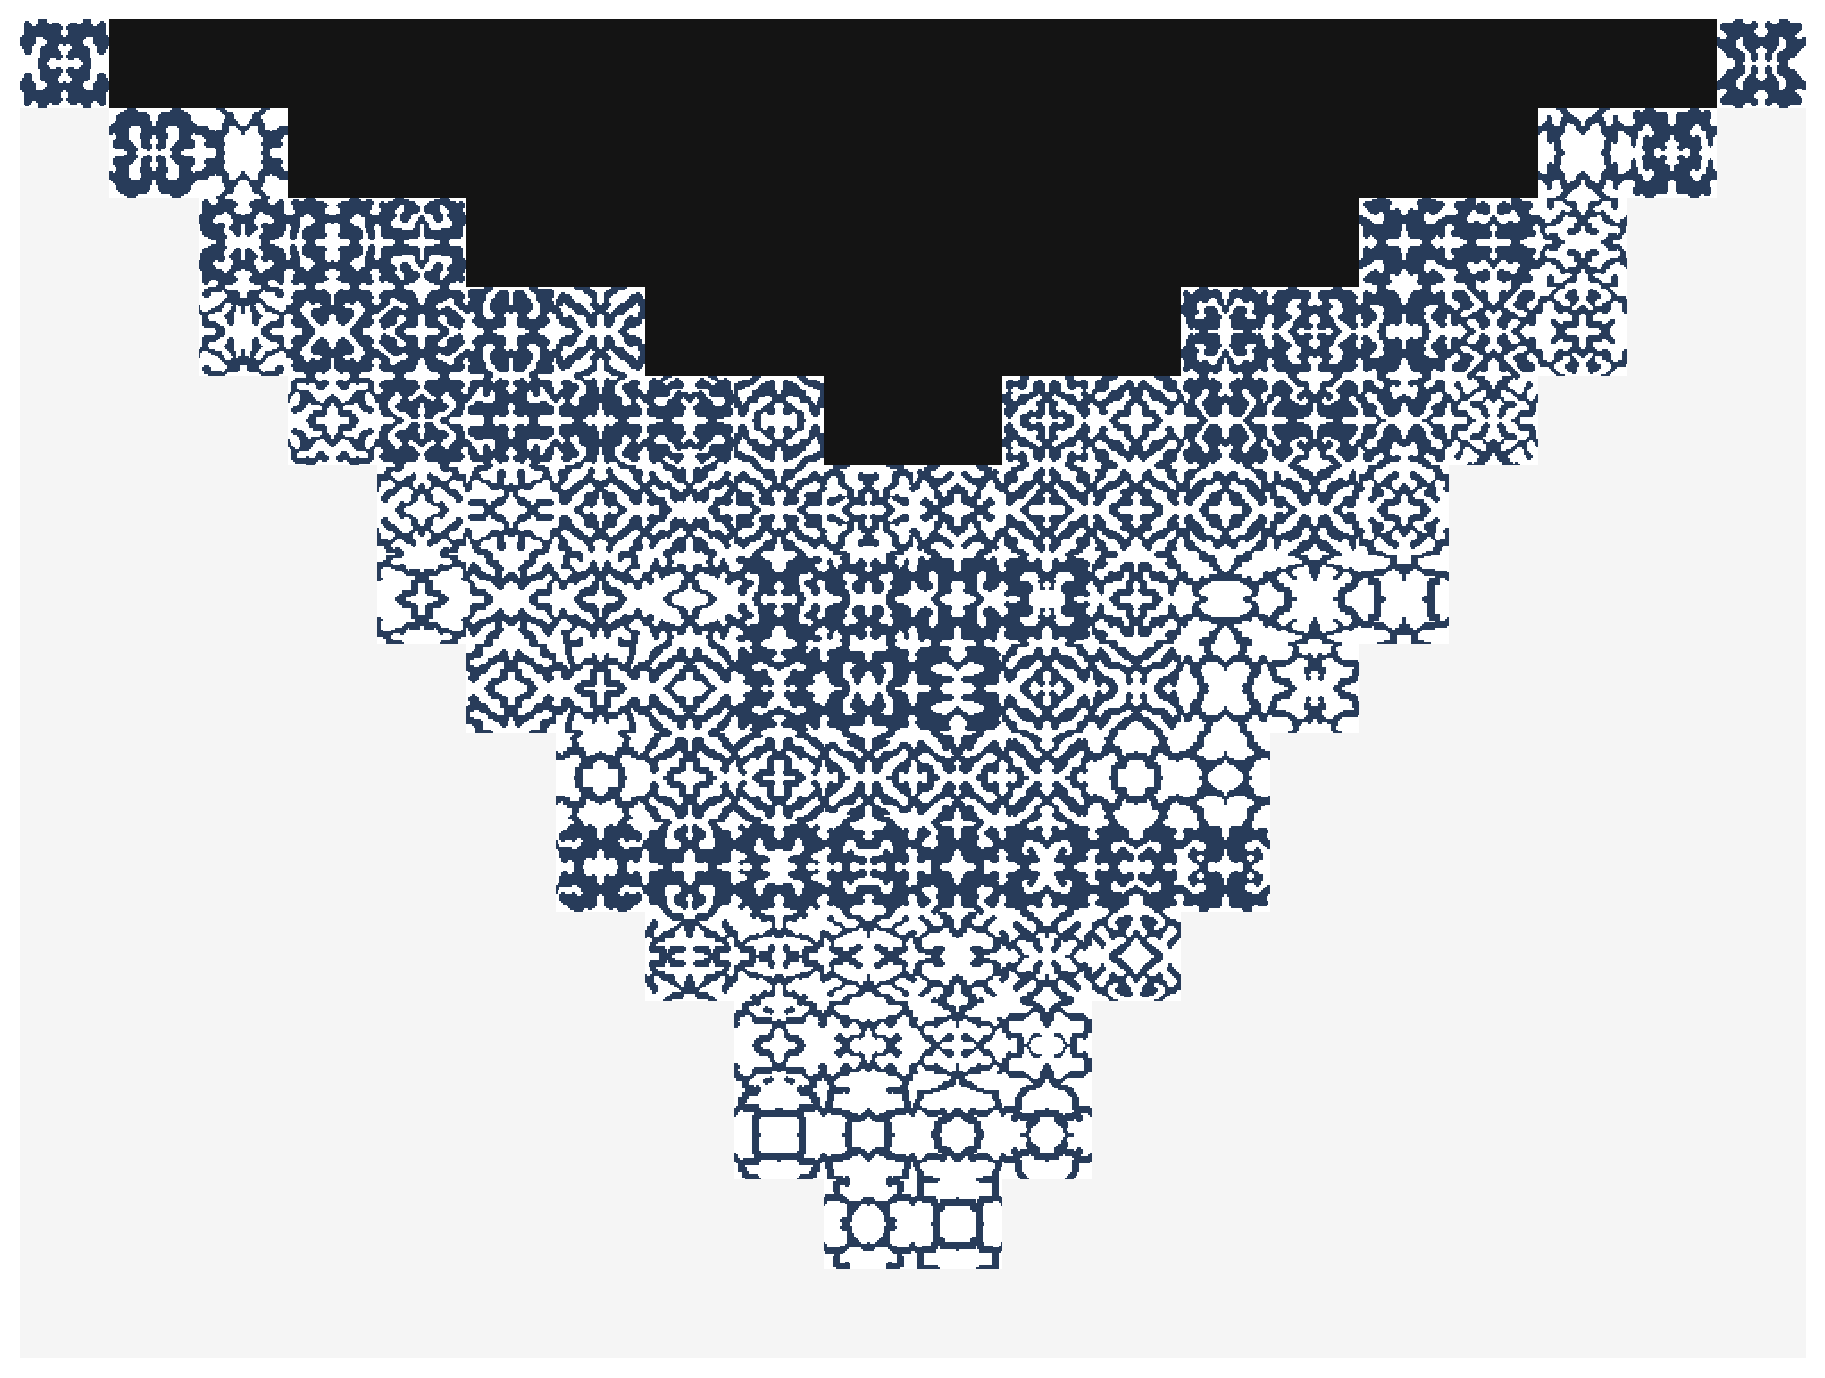
\includegraphics[width=\linewidth]{cloak_microstructure_diffusion.png}\\
      {\scriptsize Best-of-$N$ diffusion realisation of the same target field --
      visibly different, equally manufacturable patterns.}
    \end{column}
  \end{columns}
\end{frame}

% ------------------------------------------------------------
%  SLIDE 16 -- Method 4: latent-space search
% ------------------------------------------------------------
\begin{frame}{\ding{205} Method 4 -- Search in a learned latent space}
  \begin{columns}[T]
    \begin{column}{0.53\textwidth}
      \small
      Direct pixel optimisation is ill-conditioned ($\sim\!10^4$ DoFs, bad minima).
      Train an \textbf{autoencoder} on $(C,\rho,f_\star,\mcl{L})$ with a
      \emph{frequency-separated} latent
      \[
        z = z_{\mathrm{sh}} + z_f(f_\star),
      \]
      (geometry vs.\ per-frequency offset), a performance head, and a
      within-frequency contrastive ranking on $z_{\mathrm{sh}}$.
      Then \textbf{freeze} the AE and optimise the \emph{code} $z$:
      \[
        \min_z\ \alpha\max_i\mcl{L}(f_i;z)+(1-\alpha)\tfrac1N\textstyle\sum_i\mcl{L}(f_i;z),
        \ \ \alpha:1\!\to\!0.
      \]
    \end{column}
    \begin{column}{0.46\textwidth}
      \centering
      % FIGURE: material_field_AE.png  (AE-decoded C,rho field)
      \includegraphics[width=\linewidth]{material_field_AE.png}\\
      {\scriptsize AE latent decodes to structured, \emph{manufacturable} motifs.
      Cf.\ \texttt{frequency\_sweep\_vis.png}: AE $\eta\!\approx\!0.965$,
      neural-field $\approx\!0.985$.}
    \end{column}
  \end{columns}
  \takeaway{The latent search inherits the training distribution's manufacturable
    priors -- smoother layouts, fewer iterations than raw topology optimisation.}
\end{frame}

% ------------------------------------------------------------
%  SLIDE 17 -- Results III: microstructure realisation
% ------------------------------------------------------------
\begin{frame}{Results III -- how much survives fabrication?}
  \begin{columns}[T]
    \begin{column}{0.44\textwidth}
      \centering\scriptsize
      \captionof*{table}{Realising the $20\times15$ cloak (100 cells), $f^\star=2.0$}
      \begin{tabular}{@{}lc@{}}
        \toprule
        Realisation of the 100 cells & $\eta$ \\
        \midrule
        Continuous 4CM optimum        & $0.99$ \\
        \midrule
        Nearest-neighbour snap        & $0.82$ \\
        Inverse design (neural field) & $0.94$ \\
        \textbf{Diffusion (best-of-$N$)} & $\mathbf{0.97}$ \\
        \midrule
        Ideal continuous polar $\Ceff$ & $0.999$ \\
        \bottomrule
      \end{tabular}
    \end{column}
    \begin{column}{0.55\textwidth}
      \centering
      % FIGURE: micro_method_comparison_sweep.png
      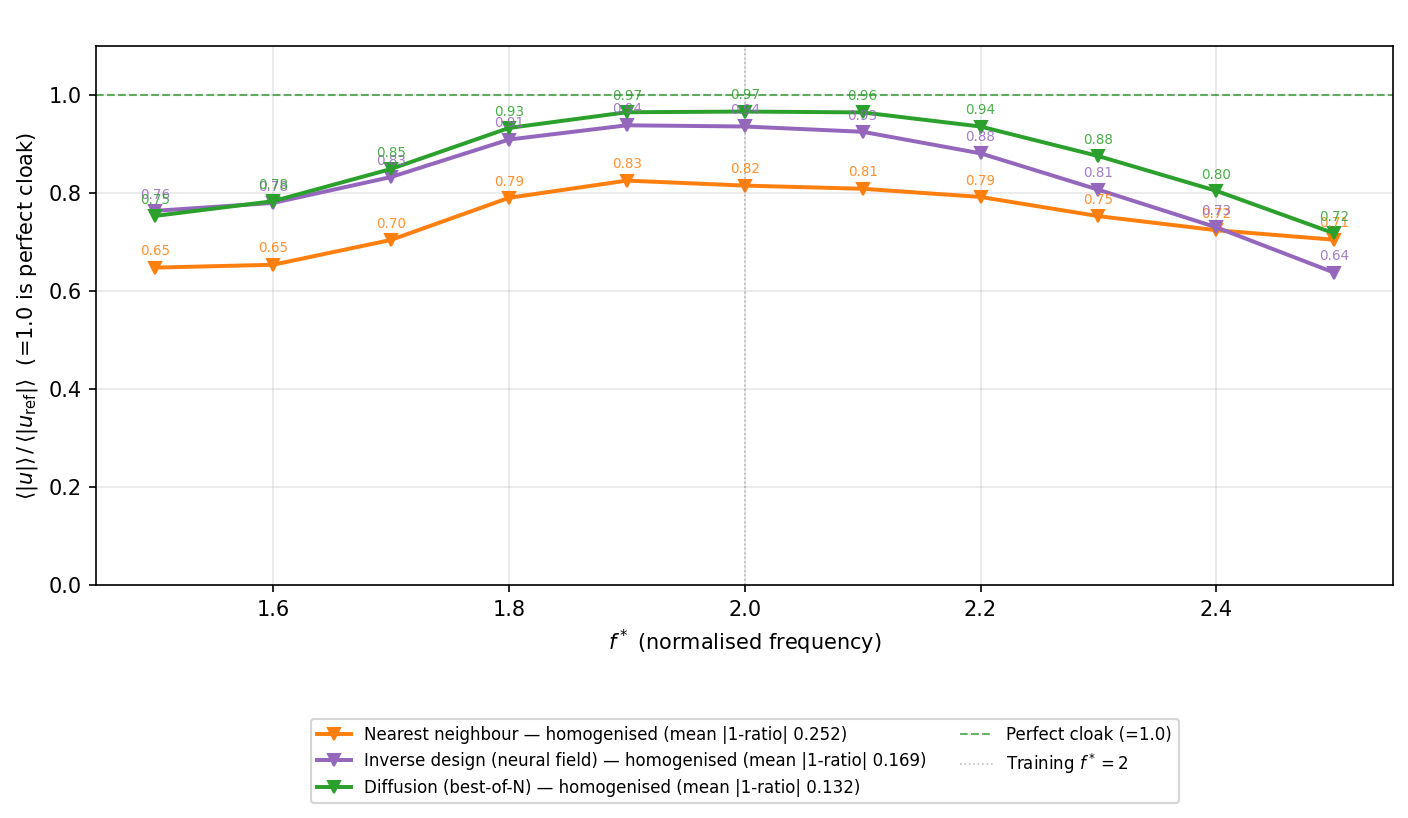
\includegraphics[width=\linewidth]{micro_method_comparison_sweep.png}\\
      {\scriptsize $\eta(f)$ across the band: diffusion (green) stays closest to
      the perfect-cloak line; smallest mean distortion.}
    \end{column}
  \end{columns}
  \takeaway{Better per-cell matching $\Rightarrow$ better cloak: best-of-$N$
    diffusion recovers \bignum{97\%}{} of the ideal, from fabricable
    single-material cells.}
\end{frame}

% ------------------------------------------------------------
%  SLIDE 18 -- Conclusions + future work
% ------------------------------------------------------------
\begin{frame}{Conclusions}
  \footnotesize
  \begin{itemize}
    \setlength{\itemsep}{0.45em}
    \item A single \textbf{differentiable pipeline} -- coordinate neural field
          $+$ JAX-FEM adjoint -- designs Rayleigh-wave carpet cloaks inside the
          realisable Cauchy class.
    \item \textbf{Near-perfect} single-frequency ($\eta=0.99$) and \textbf{broadband}
          ($\approx0.96$ over an octave) cloaking, beating closed-form
          symmetrisation.
    \item Four ML routes to a real structure -- neural-field optimisation,
          inverse design, guided diffusion, latent search -- with
          \textbf{diffusion recovering $\approx97\%$} of ideal performance from a
          \emph{single} constituent.
  \end{itemize}
  \vspace{0.6em}
  \begin{beamercolorbox}[wd=\textwidth, rounded=true, sep=7pt]{block body alerted}
    \textbf{\textcolor{ASTRAnavy}{Future work:}}
    \textcolor{ASTRAnavy}{\footnotesize a differentiable generative manifold queried
    \emph{during} optimisation; multiscale generation with connected neighbours on a
    body-fitted mesh; 3-D cloaks; and polar/Cosserat microstructures to close the
    broken-minor-symmetry gap.}
  \end{beamercolorbox}
\end{frame}

% ------------------------------------------------------------
%  SLIDE 19 -- References
% ------------------------------------------------------------
\begin{frame}{References}
  \footnotesize
  \begin{thebibliography}{9}
    \setbeamertemplate{bibliography item}[text]
    \bibitem{brun2009} Brun, Guenneau, Movchan (2009).
      \textit{Achieving control of in-plane elastic waves.} Appl.\ Phys.\ Lett.
    \bibitem{norris2011} Norris, Shuvalov (2011).
      \textit{Elastic cloaking theory.} Wave Motion.
    \bibitem{nassar2018} Nassar, Chen, Huang (2018).
      \textit{Polar metamaterials for elastic cloaking.} (Cosserat lattice).
    \bibitem{chatzopoulos2023} Chatzopoulos et al.\ (2023).
      \textit{Symmetrised Rayleigh-wave carpet cloaks.} (baseline).
    \bibitem{wang2022} Wang et al.\ (2022).
      \textit{Database-selected orthotropic mechanical cloaks.}
    \bibitem{tancik2020} Tancik et al.\ (2020).
      \textit{Fourier features let networks learn high-frequency functions.}
    \bibitem{nakarmi2024} Nakarmi et al.\ (2024).
      \textit{Cellular-automaton generation of mesostructure libraries.}
    \bibitem{yang2024} Yang et al.\ (2024).
      \textit{Guided diffusion for inverse microstructure design.}
    \bibitem{xu2020jaxfem} Xu et al.\ (2020).
      \textit{JAX-FEM: a differentiable finite-element solver.}
  \end{thebibliography}
  \par\vspace{0.3em}{\scriptsize\itshape (Placeholder entries -- replace with the
  paper's \texttt{cas-refs.bib} for the final deck.)}
\end{frame}

% ------------------------------------------------------------
%  SLIDE 20 -- Thank You
% ------------------------------------------------------------
\thankyouslide{%
  \textit{The authors gratefully acknowledge Danila Rukhovich (Google) for support.} 
  \textit{Code, dataset, and the differentiable JAX-FEM pipeline available on GitHub https://github.com/M3LLab/nn-cloaking}
  }

% ============================================================
\end{document}
% ============================================================
